\documentclass{svproc}
%
% RECOMMENDED %%%%%%%%%%%%%%%%%%%%%%%%%%%%%%%%%%%%%%%%%%%%%%%%%%%
%
%%%% Standard Packages
%%<additional latex packages if required can be included here>
\usepackage{graphicx}%
\usepackage{multirow}%
\usepackage{amsmath,amssymb,amsfonts}%
\usepackage{mathrsfs}%
\usepackage[title]{appendix}%
\usepackage{xcolor}%
\usepackage{textcomp}%
\usepackage{manyfoot}%
\usepackage{booktabs}%
\usepackage{algorithm}%
\usepackage{algorithmicx}%
\usepackage{algpseudocode}%
\usepackage{listings}%
\usepackage{tikz}
% to typeset URLs, URIs, and DOIs
\usepackage{url}
\usepackage{adjustbox}
\usepackage{textcomp}
\usepackage{hyperref} 

\usetikzlibrary{arrows,automata}

\def\UrlFont{\rmfamily}
\def\orcidID#1{\unskip$^{[#1]}$} % added MR 2018-03-10

\lstset{
    basicstyle=\ttfamily,
    breaklines=true,
    frame=single,
    language=HTML,
    showstringspaces=false,
    commentstyle=\color{gray},
    keywordstyle=\color{blue},
    stringstyle=\color{red},
    upquote=true
}

\begin{document}
\mainmatter              % start of a contribution
%
\title{Directed Graph Hashing}
%
\titlerunning{Directed Graph Hashing}  % abbreviated title (for running head)
%                                     also used for the TOC unless
%                                     \toctitle is used
%
\author{Caleb Helbling\inst{1}\orcidID{abc}}
%
\authorrunning{Caleb Helbling} % abbreviated author list (for running head)
%

\institute{Draper, 555 Technology Square, Cambridge, MA USA 02139,\\
\email{chelbling@draper.com},\\ WWW home page:
\texttt{https://helbl.ing/}}

\maketitle              % typeset the title of the contribution

\begin{abstract}
%The abstract should summarize the contents of the paper
%using at least 70 and at most 150 words. It will be set in 9-point
%font size and be inset 1.0 cm from the right and left margins.
%There will be two blank lines before and after the Abstract. 

This paper presents several algorithms for hashing directed graphs. We distinguish between the cases of assigning a hash value for a digraph as a whole vs hashing specific nodes within a graph. In our algorithm design we are careful to take into account symmetry within a digraph by computing vertex orbits and the automorphism group. Nodes that are identical modulo symmetry are assigned equal hashes. We also present a Merkle-style hashing algorithm that seeks to fulfill the recursive principle that a hash of a node should only depend on the hash of its neighbors. Our algorithms work even in the presence of cycles, which would not be possible with a naive recursive approach. Structurally hashing trees has seen widespread use in blockchain, source code version control, and web applications. Despite the popularity of tree hashing, directed graph hashing remains unstudied in the literature.

% We would like to encourage you to list your keywords within
% the abstract section using the \keywords{...} command.
\keywords{keyword1, keyword2, keyword3}
\end{abstract}
%
\section{Introduction}\label{sec1}
%

Hashing functions are fundamental primitives in the modern software stack. They are used in data storage and retrieval, digital fingerprint, checksum, and cryptographic applications. Traditionally, hash functions take as input bit strings of arbitrary length and return a bit string of a fixed size $\mathcal{H} : \{0,1\}^* \rightarrow \{0,1\}^n$. Good hashing functions should be fast to compute, minimize the chance of duplication of output values, and produce large changes in output for small changes in input. Over the years, many bit string hashing functions have been created, including MD5 \cite{md5}, SHA-2 \cite{sha2}, and SHA-3 \cite{sha3}.

\begin{algorithm}
\caption{Recursive Merkle-tree Hashing of Ordered Binary Tree}
\[
\text{mh}(n) =
\begin{cases} 
    \mathcal{H}(n.\text{label}) & n \text{ is a leaf} \\
    \mathcal{H}(n.\text{label} \text{+} \text{mh}(n.\text{left}) \text{+} \text{mh}(n.\text{right})) & \text{otherwise}
\end{cases}
\]
\label{alg:merklehashing}
\end{algorithm}

Hashing functions can be extended to trees via a simple extension of Merkle hashing \cite{merkle1987digital}. In Merkle tree hashing, the hash of a node is computed by hashing the concatenation of the node's label with the recursive hash of the node's children. Algorithm \ref{alg:merklehashing} gives a simple recursive implementation of Merkle tree hashing for ordered binary trees. This variation of Merkle hashing has seen use in many applications, including cryptocurrency \cite{bitcoin}, version control systems \cite{git}, and distributed hypertext document storage systems \cite{ipfs}.

Hashing directed graphs adds an additional layer of complexity not present in trees. Directed graphs can have arbitrary cycles, which prevents the use of naive recursion. We work around this issue via two different prongs. First, we make use of graph canonization algorithms, which can be used to give a unique order to the nodes. This order can be used to output an adjacency list, which can then be hashed with an ordinary string hashing function. Second, we use the structure of the graph condensation, which is an induced acyclic graph and therefore amenable to recursion.

Our contributions in this paper can therefore be described as follows:

\begin{itemize}
    \item We give an algorithm for hashing an entire directed graph using graph canonization.
    \item We give an algorithm for hashing specific nodes within a digraph. This approach takes into account any symmetry present within the graph.
    \item We give quadratic time algorithms for hashing based on depth-first search in the special case where outgoing node edges are strictly ordered.
    \item We outline a recursive approach for hashing cyclic directed graphs, drawing inspiration from Merkle-tree hashing. Although this approach cannot be used to fingerprint graphs in a global sense, we will make a bisimulation argument from the perspective of an observer traversing a graph that this approach is sufficient for many use cases.
\end{itemize}

\section{Background}

\begin{figure}[t]  
\centering 
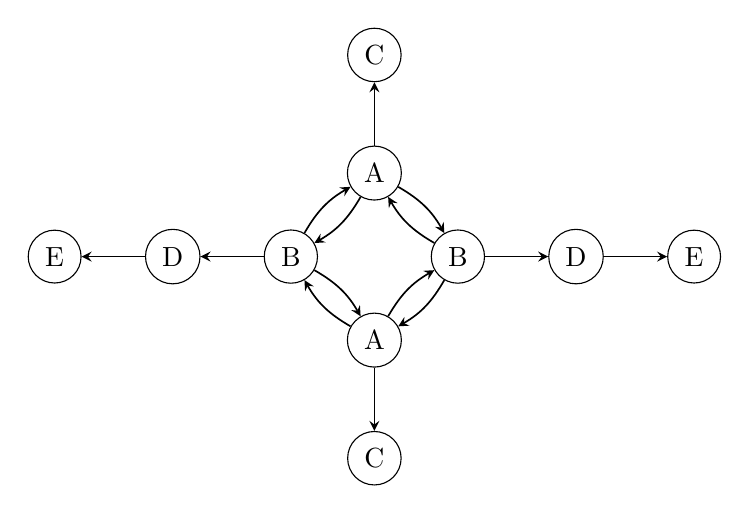
\begin{tikzpicture}[
    > = stealth, % arrow head style
    shorten > = 0pt, % don't touch arrow head to node
    auto,
    node distance = 1.5cm, % distance between nodes
    semithick % line style
]
\tikzstyle{every state}=[
    draw = black,
    thin,
    fill = white,
    minimum size = 6mm
]

\node[state] (a) {A};
\node[state] (b) [below left of=a] {B};
\node[state] (c) [below right of=a] {B};
\node[state] (d) [below right of=b] {A};
\node[state] (e) [above of=a] {C};
\node[state] (f) [below of=d] {C};
\node[state] (g) [right of=c] {D};
\node[state] (h) [right of=g] {E};
\node[state] (i) [left of=b] {D};
\node[state] (j) [left of=i] {E};

\path[->] (a) edge [bend left=15] node {} (b);
\path[->] (a) edge [bend left=15] node {} (c);
\path[->] (c) edge [bend left=15] node {} (d);
\path[->] (b) edge [bend left=15] node {} (d);

\path[<-] (a) edge [bend right=15] node {} (b);
\path[<-] (a) edge [bend right=15] node {} (c);
\path[<-] (b) edge [bend right=15] node {} (d);
\path[<-] (c) edge [bend right=15] node {} (d);

\path[->] (d) edge node {} (f);
\path[->] (a) edge node {} (e);
\path[->] (c) edge node {} (g);
\path[->] (g) edge node {} (h);
\path[->] (b) edge node {} (i);
\path[->] (i) edge node {} (j);

\end{tikzpicture}
\caption{This directed graph contains five orbits, identified by the letters A, B, C, D and E. Nodes within the same orbit are structurally identical due to the symmetry of the directed graph.}
\label{fig:orbitexample}
\end{figure}

We now give some basic graph theory definitions required for this paper, but which a more general audience interested in hashing may not be informed about. An \textit{automorphism} of some graph $G=(V,E,L)$ is defined as a permutation $\sigma$ of vertices such that $(u, v) \in E$ if and only if $(\sigma(u), \sigma(v)) \in E$. Here $L$ is a labeling function that maps vertices to strings. Informally, the automorphism group gives all of the ways that $G$ is symmetrical.

\[
\text{Aut}(G) = \{ \sigma : V \rightarrow V \mid (u, v) \in E \leftrightarrow (\sigma(u), \sigma(v)) \in E\}
\]

A \textit{vertex orbit} is the equivalence class of vertices of a graph under the action of automorphisms. Informally, the orbit of a vertex $v$ can be thought of as the set of vertices that are symmetrically identical to $v$. Figure \ref{fig:orbitexample} gives an example of how orbits can be used to partition a graph.

\[
\text{Orb}(v,G) = \{u \in V \mid \exists \sigma \in \text{Aut}(G) \text{ such that } \sigma(v) = u\}
\]

\textit{Canonical labeling} is the process of ordering graph vertices such that isomorphic graphs canonize to the same value. Note that canonical labeling algorithms cannot distinguish between different graph automorphisms. Algorithms that can compute canonical labels are widely used in practice for graph isomorphism testing. Some examples of canonical labeling algorithms include nauty \cite{nauty}, bliss \cite{bliss}, and saucy \cite{saucy}.

\begin{figure}[t]
  \centering
  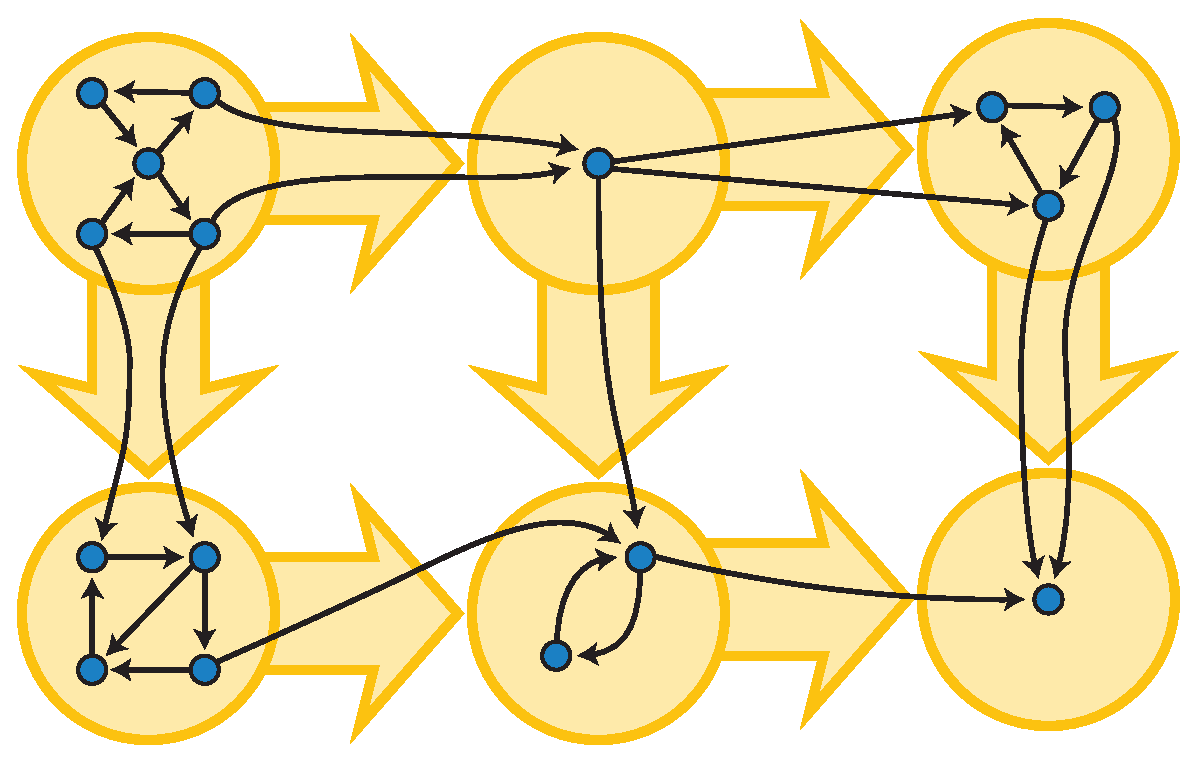
\includegraphics[width=0.5\linewidth]{Fig2.eps}
  \caption{Each yellow node contains a strongly connected component of a graph. When each strongly connected component is contracted into a single node, the yellow condensation graph is formed. Public domain figure courtesy of David Eppstein.}
  \label{fig:condensation}
\end{figure}

The recursive Merkle-style algorithm will utilize the analysis of cycles within a directed graph. A \textit{strongly connected component} of a graph is a maximal set of vertices such that there exists a path in the graph between any two vertices within the strongly connected component. A \textit{condensation graph} is formed by contracting strongly connected components into single nodes. We will exploit the acyclicity of the condensation graph to construct our recursive algorithm. Figure \ref{fig:condensation} shows an example of strongly connected components and the induced condensation graph.

\section{Algorithms}

\subsection{Canonization for Graph Hashing}

\begin{algorithm}
    \caption{Directed Graph Hash}\label{digraphhash}
    \begin{algorithmic}[1]
    \Function{$\mathcal{H_G}$}{G=(V,E,L)}
        \State \Comment{V is the set of vertices, E is the set of edges, L is the node labeling function}
        \State $\rho \gets$ \textproc{canonize}($G$) \Comment{\textproc{canonize} returns a mapping from vertices to their location in the canonical order}
        \State adj\_list $\gets$ \textproc{sort}($[(\rho(u), \rho(v)) \mid (u,v) \in E]$)
        \State labels $\gets$ [L($\rho^{-1}(n)$) \textbf{for} n \textbf{in} 0..\textbar V\textbar]
        \State \Return $\mathcal{H}$(\textproc{to\_str}((labels, adj\_list)))
    \EndFunction
    \end{algorithmic}
\end{algorithm}

We now distinguish between creating a hash for a graph and hash for a node in a graph. Hashing a graph should give a unique fingerprint to the graph as a whole, whereas the hash of a node should also needs to ``point to'' a single specific node within the graph.

The strongest property we can prove about a graph hashing algorithm is the uniqueness of hash values modulo isomorphism. To be more precise, the hash of a graph $\mathcal{H_G}$ has the property $\mathcal{H_G}(G_1)=\mathcal{H_G}(G_2)$ if and only if $G_1 \cong G_2$. Extending this idea to nodes, $\mathcal{H_N}(v_1, G_1)=\mathcal{H_N}(v_2, G_2)$ if and only if $G_1 \cong G_2$, $\exists \phi . v_2 \in \text{Orb}(\phi(v_1), G_2)$, and $\exists \phi . v_1 \in \text{Orb}(\phi^{-1}(v_2), G_1)$ where $\phi : V_1 \rightarrow V_2$ is an isomorphism from $G_1$ to $G_2$. In other words, nodes should hash to the same value if they come from isomorphic graphs, and they are identical modulo vertex orbits.

To achieve these correctness properties, we build on top of the well known string hashing functions and canonical labeling algorithms. We begin by canonizing the input digraph and constructing an adjacency list sorted in canonical order. The node labels (in canonical order) and the canonized adjacency list are then encoded as strings and hashed using a string hashing function $\mathcal{H}$. Algorithm \ref{digraphhash} gives an implementation of this approach.

To achieve these properties, we build off the string hashing functions and canonical labeling algorithms. Hashing an entire graph is straightforward and begins by canonizing the entire digraph. The adjacency list (sorted using the canonical order) and the vertex labels (ordered using the canonical order) are represented as strings and hashed using a string hashing function $\mathcal{H}$. Algorithm \ref{digraphhash} gives an implementation of this approach. Note that the return value of the canonize function is a mapping from the vertices of the input to the canonical order.

\begin{theorem}[Proof of Correctness]
\label{thm:digraphhashcorrect}
Assuming that the string hashing function $\mathcal{H}$ is injective, $\mathcal{H_G}(G_1)=\mathcal{H_G}(G_2)$ if and only if $G_1 \cong G_2$.
\end{theorem}

\begin{proof}
($\Rightarrow$)If $\mathcal{H_G}(G_1)=\mathcal{H_G}(G_2)$, then the canonized adjacency list/vertex label lists are identical. If these representations of $G_1$ and $G_2$ are identical, then $G_1$ and $G_2$ have identical canonical form $G_3$. This means that $G_1 \cong G_3$ and $G_2 \cong G_3$, which implies that $G_1 \cong G_2$ by transitivity.

%Of course real string hashing functions are not injective by the pigeonhole principle, however in practice nobody has yet found collisions for algorithms such as SHA512. Therefore for this approach we treat string hashing algorithms as injective. The identity function or an asymmetric encryption algorithm are examples of truly injective string transformation functions, so those could be used as alternatives if desired.

($\Leftarrow)$ Let $G_3$ be the output graph of canonizing $G_1$, and $G_4$ be the output of canonizing graph $G_2$. Since $G_1 \cong G_2$, we conclude that $G_3=G_4$ since isomorphic graphs canonize to the same graph. This implies that the sorted adjacency lists and ordered vertex label lists are equivalent, so the string representation is equivalent. Therefore the string hash output are equivalent as well, which shows that $\mathcal{H_G}(G_1)=\mathcal{H_G}(G_2)$.

\qed
\end{proof}

\begin{algorithm}
    \caption{Directed Graph Node Hash}\label{digraphnodehash}
    \begin{algorithmic}[1]
    \Function{$\mathcal{H_N}$}{v, G}
        \State $\rho \gets$ \textproc{canonize}(G)
        \State g\_hash $\gets \mathcal{H_G}(G)$
        \State orbit\_idx $\gets$ $\min(\text{Orb}(\rho(v),\rho(G)))$
        \State \Return $\mathcal{H}$(\textproc{to\_str}((orbit\_idx, g\_hash)))
    \EndFunction
    \end{algorithmic}
\end{algorithm}

The algorithm for hashing nodes in a graph builds on the algorithm for hashing graphs. First, the graph is canonized and the hash of the entire canonical graph is computed using Algorithm \ref{digraphhash}. Then we compute the orbit index of the input vertex, which is defined to be the canonical index of the equivalence class representative element, where the equivalence relation in this case is the vertex orbit. The orbit index and the graph hash are then combined and passed through a string hashing function.

\begin{theorem}[Proof of Correctness]
\label{thm:digraphnodehashcorrect}
$\mathcal{H_N}(v_1, G_1)=\mathcal{H_N}(v_2, G_2)$ if and only if $G_1 \cong G_2$, $\exists \phi . v_2 \in \text{Orb}(\phi(v_1), G_2)$, and $\exists \phi . v_1 \in \text{Orb}(\phi^{-1}(v_2), G_1)$ where $\phi : V_1 \rightarrow V_2$ is an isomorphism between $G_1$ and $G_2$.
\end{theorem}

\begin{proof}
($\Rightarrow$) If $\mathcal{H_N}(v_1, G_1)=\mathcal{H_N}(v_2, G_2)$, then the orbit index of $v_1$ in $\mathcal{H_N}(v_1, G_1)$ is equal to the orbit index of $v_2$ in $\mathcal{H_N}(v_2, G_2)$, and $\mathcal{H_G}(G_1)=\mathcal{H_G}(G_2)$ by the injectivity of string hashing. Then by Theorem \ref{thm:digraphhashcorrect}, $G_1 \cong G_2$.

Let $\rho_1$ be the canonization of $G_1$ and $\rho_2$ be the canonization of $G_2$. Then $\rho_1(G_1)=\rho_2(G_2)$ since $G_1 \cong G_2$. Note that $\rho_1$ and $\rho_2$ are both isomorphisms. Then let $\phi=\rho_2^{-1} \circ \rho_1$ and $\phi^{-1}=\rho_1^{-1} \circ \rho_2$. Applying this definition of $\phi$, we wish to show that $v_2 \in \text{Orb}(\rho_2^{-1}(\rho_1 (v_1)), G_2)$ and $v_1 \in \text{Orb}(\rho_1^{-1}(\rho_2 (v_2)), G_1)$. Applying the isomorphisms $\rho_2$ and $\rho_1$ to these sets respectively, this is equivalent to showing that $\rho_2(v_2) \in \text{Orb}(\rho_1 (v_1), \rho_2(G_2))$ and $\rho_1(v_1) \in \text{Orb}(\rho_2 (v_2), \rho_1(G_1))$.

Recall that the orbit index of $v_1$ in $\mathcal{H_N}(v_1, G_1)$ is equal to the orbit index of $v_2$ in $\mathcal{H_N}(v_2, G_2)$. This implies that the two orbit sets are equal $\text{Orb}(\rho_1 (v_1), \rho_1(G_1))=\text{Orb}(\rho_2 (v_2), \rho_2(G_2))$ since they have equal representative elements. Then since $\rho_1(G_1)=\rho_2(G_2)$, $\text{Orb}(\rho_1 (v_1), \rho_1(G_1))=\text{Orb}(\rho_2 (v_2), \rho_2(G_2))=\text{Orb}(\rho_1 (v_1), \rho_2(G_2))$\\
$=\text{Orb}(\rho_2 (v_2), \rho_1(G_1))$. Then trivially $\rho_1(v_1) \in \text{Orb}(\rho_1 (v_1), \rho_1(G_1))$ and $\rho_2(v_2) \in \text{Orb}(\rho_2 (v_2), \rho_2(G_2))$. Following the chain of equalities and making the appropriate substitutions, then $\rho_2(v_2) \in \text{Orb}(\rho_1 (v_1), \rho_2(G_2))$ and $\rho_1(v_1) \in \text{Orb}(\rho_2 (v_2), \rho_1(G_1))$.

($\Leftarrow$) If $G_1 \cong G_2$, then $\mathcal{H_G}(G_1)=\mathcal{H_G}(G_2)$ by Theorem \ref{thm:digraphhashcorrect}. Then there exists some isomorphism $\phi$ and $\phi'$ such that $v_2 \in \text{Orb}(\phi(v_1),G_2)$ and $v_1 \in \text{Orb}(\phi'^{-1}(v_2),G_1)$. Let $\rho_1$ be the canonization of $G_1$ and $\rho_2$ be the canonization of $G_2$. Applying these isomorphisms, we have $\rho_2(v_2) \in \text{Orb}(\rho_2(\phi(v_1)), \rho_2(G_2))$ and $\rho_1(v_1) \in \text{Orb}(\rho_1(\phi'^{-1}(v_2)),\rho_1(G_1))$. Let $f=\rho_1 \circ \phi^{-1} \circ \rho_2^{-1}$ and $f'=\rho_2 \circ \phi' \circ \rho_1^{-1}$ be automorphisms over the canonized graph.

Then by definition of orbit, $\text{Orb}(\rho_2(\phi(v_1)), \rho_2(G_2))=\text{Orb}(f(\rho_2(\phi(v_1))), \rho_2(G_2))$ and $\text{Orb}(\rho_1(\phi'^{-1}(v_2)),\rho_1(G_1)) = \text{Orb}(f'(\rho_1(\phi'^{-1}(v_2)),\rho_1(G_1)))$. Substituting in the definitions of $f$ and $f'$, we have $\text{Orb}(\rho_2(\phi(v_1)), \rho_2(G_2))=\text{Orb}(\rho_1(v_1), \rho_2(G_2))$ and $\text{Orb}(\rho_1(\phi'^{-1}(v_2)),\rho_1(G_1)) = \text{Orb}(\rho_2(v_2),\rho_1(G_1))$. This shows that $\rho_2(v_2) \in \text{Orb}(\rho_1(v_1), \rho_2(G_2))$ and $\rho_1(v_1) \in \text{Orb}(\rho_2(v_2),\rho_1(G_1))$. Since $G_1 \cong G_2$, $\rho_1(G_1)=\rho_2(G_2)$ so $\rho_2(v_2) \in \text{Orb}(\rho_1(v_1), \rho_1(G_1))$ and $\rho_1(v_1) \in \text{Orb}(\rho_2(v_2),\rho_2(G_2))$. This suffices to show that the orbit indices of are equal in the computations of $\mathcal{H_N}(v_1, G_1)$ and $\mathcal{H_N}(v_2, G_2)$.

Since the orbit indices are equal and $\mathcal{H_G}(G_1)=\mathcal{H_G}(G_2)$, then $\mathcal{H_N}(v_1, G_1)=\mathcal{H_N}(v_2, G_2)$.

\qed
\end{proof}

\subsection{Outgoing Ordered Edge Graphs}

For many real world applications of graph hashing, the labels on a node's outgoing edges are strictly ordered. As an example, consider a scenario in which we are hashing hyperlinked HTML web pages for a content-addressable system. Each node in our graph is an individual page, and there is a strict order for outgoing edges (hyperlinks) based on the order in which the links appear in the HTML tree.

We can take advantage of this extra structure on the edges to create a node hashing algorithm that runs in polynomial time and neatly encapsulates the idea thtat the hash of a node should depend only the reachable subgraph structure. Algorithm \ref{alg:node-outgoing-edges} gives an overview of this approach based on the traversal order of a depth-first search. Note that the algorithms given in this section are directly inspired by the more general Scott graph canonization algorithm given by Bloyet, Marteau and Fr\'enod \cite{scott}.

\begin{algorithm}[H]
    \label{alg:node-outgoing-edges}
    \caption{Node Hash - Outgoing Ordered Edges}\label{alg:dfs-node-hash}
    \begin{enumerate}
        \item For some input node $n$, perform a depth first search starting at $n$ and record the visitation order of the reachable nodes.
        \item Construct an adjacency list where the node identifiers are given by the visitation order. Sort this adjacency list lexicographically.
        \item Create a list of labels in the order given by the DFS visitation.
        \item Hash the combined adjacency and label list to compute the hash of $n$.
    \end{enumerate}    
\end{algorithm}

We take a similar approach in Algorithm \ref{alg:scc-outgoing-edges} to compute the canonical order and orbit partition of a strongly connected outgoing edge ordered digraph in quadratic time.

\begin{algorithm}[H]
    \label{alg:scc-outgoing-edges}
    \caption{Canonization and Orbit Partitioning for Strongly Connected Outgoing Ordered Edge Graphs}\label{alg:dfs-scc-hash}
    \begin{enumerate}
        \item For each node $n$:
        \begin{enumerate}
          \item Perform a depth first search starting at $n$ and record the visitation order of the reachable nodes.
          \item Construct an adjacency list of the edges using the visitation order. The elements of the pairs of this adjacency list are natural numbers refering to visitation order.
          \item Construct a list of labels of nodes in the graph where the order is given by the visitation order.
          \item Define the \textit{DFS label} as the pair of the adjacency list and label list.
        \end{enumerate}
        \item Canonize the graph by sorting the nodes by their \textit{DFS label} lexicographically.
        \item Nodes in the same orbit will have identical \textit{DFS label} values. \textbf{Proof}: It is easy to construct an automorphism between two nodes in the original graph using the \textit{DFS label}.
        \item At this point we now have a canonical order and orbit partition that can be used in Algorithm \ref{digraphhash} or \ref{digraphnodehash}.
    \end{enumerate}
\end{algorithm}

\begin{figure}[t]  
\centering 
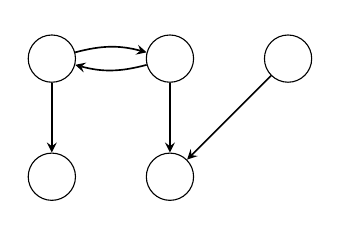
\begin{tikzpicture}[
    > = stealth, % arrow head style
    shorten > = 0pt, % don't touch arrow head to node
    auto,
    node distance = 1.5cm, % distance between nodes
    semithick % line style
]
\tikzstyle{every state}=[
    draw = black,
    thin,
    fill = white,
    minimum size = 6mm
]

\node[state] (a) {};
\node[state] (b) [right of=a] {};
\node[state] (c) [below of=a] {};
\node[state] (d) [below of=b] {};
\node[state] (e) [right of=b] {};

\path[->] (a) edge [bend left=15] node {} (b);
\path[<-] (a) edge [bend right=15] node {} (b);

\path[->] (a) edge node {} (c);
\path[->] (b) edge node {} (d);

\path[->] (e) edge node {} (d);

\end{tikzpicture}
\caption{The symmetry of the bottom two nodes is broken only by considering the incoming edges from higher in the graph. In this case the two bottom nodes are no longer in the same orbit.}
\label{fig:breaksymmetry}
\end{figure}

Why must we restrict ourselves to the special case of strongly connected graphs? In the case of a generic digraph, the symmetry and therefore the orbit of a node depends not only on the structure of the reachable subgraph, but also on the structure from ancestor nodes. Incoming edges from ancestor nodes can break the symmetry of an orbit, as demonstrated in Figure \ref{fig:breaksymmetry}. In the case of a strongly connected graph, we do not encounter this issue as all nodes are mutual descendants of one another.

\subsection{Merkle Graph Hashing}

\begin{algorithm}
    \caption{Merkle Graph Node Hashing}\label{alg:merklegraphhash}
    \begin{algorithmic}[1]
    \Function{$\mathcal{H_{NM}}$}{v,G=(V,E,L)}
        \State $S \gets$ \textproc{Scc}(v,$G$) \Comment{$S$ is the set of vertices in the SCC containing v}
        \State $L'(u)=\textproc{to\_str}((L(u),\textproc{sort}([\mathcal{H_{NM}}(w,G) \mid u \in S \land w \notin S \land (u,w) \in E])))$ \\ \Comment{Relabel all nodes in the SCC using the recursively computed hashes}
        \State $(V', E', L'') \gets$ \textproc{Subgraph}(S, $G$)
        \State $G' \gets (V',E',L')$
        \State \Return $\mathcal{H_N}(v, G')$ \Comment{Hash the relabelled SCC containing v}
    \EndFunction
    \end{algorithmic}
\end{algorithm}

\section{Application Sketch}

\begin{figure}
\label{fig:webpage-example}
\centering

% Row 1: Original HTML snippets
\textbf{Row 1: Original HTML Pages}

\vspace{0.3cm}

\begin{adjustbox}{max width=\textwidth}
\begin{tabular}{p{5.5cm}@{\hspace{0.3cm}}p{5.5cm}@{\hspace{0.3cm}}p{5.5cm}}
index.html
\begin{lstlisting}[language=HTML]
<body>
  <h1>Welcome</h1>
  <a href="about.html">
    About Us
  </a>
  <a href="http://e.com">
    External Resource
  </a>
</body>
\end{lstlisting}
&
about.html
\begin{lstlisting}[language=HTML]
<body>
  <h1>About Us</h1>
  <a href="index.html">
    Home
  </a>
  <a href="contact.html">
    Contact
  </a>
  <a href="http://p.com">
    Partner Site
  </a>
</body>
\end{lstlisting}
&
contact.html
\begin{lstlisting}[language=HTML]
<body>
  <h1>Contact Us</h1>
  <a href="about.html">
    About
  </a>
  <a href="http://e.com">
    External Resource
  </a>
</body>
\end{lstlisting}
\end{tabular}
\end{adjustbox}

\vspace{0.5cm}

% Row 2: Tokenized/Hashed HTML snippets
\textbf{Row 2: Replace intra-SCC links with natural numbers, recursively hash inter-SCC links}

\vspace{0.3cm}

\begin{adjustbox}{max width=\textwidth}
\begin{tabular}{p{5.5cm}@{\hspace{0.3cm}}p{5.5cm}@{\hspace{0.3cm}}p{5.5cm}}
index.html
\begin{lstlisting}[language=HTML]
<body>
 <h1>Welcome</h1>
 <a href="{0}">
  About Us
 </a>
 <a href="#8ab43f">
  External Resource
 </a>
</body>
\end{lstlisting}
&
about.html
\begin{lstlisting}[language=HTML]
<body>
 <h1>About Us</h1>
 <a href="{0}">
  Home
 </a>
 <a href="{1}">
  Contact
 </a>
 <a href="#f2d91c">
  Partner Site
 </a>
</body>
\end{lstlisting}
&
contact.html
\begin{lstlisting}[language=HTML]
<body>
  <h1>Contact Us</h1>
  <a href="{0}">
    About
  </a>
  <a href="#8ab43f">
    External Resource
  </a>
</body>
\end{lstlisting}
\end{tabular}
\end{adjustbox}

\vspace{0.5cm}

% Row 3: Graph representation
\textbf{Row 3: Construct directed graph (labels taken from previous row)}

\vspace{0.3cm}

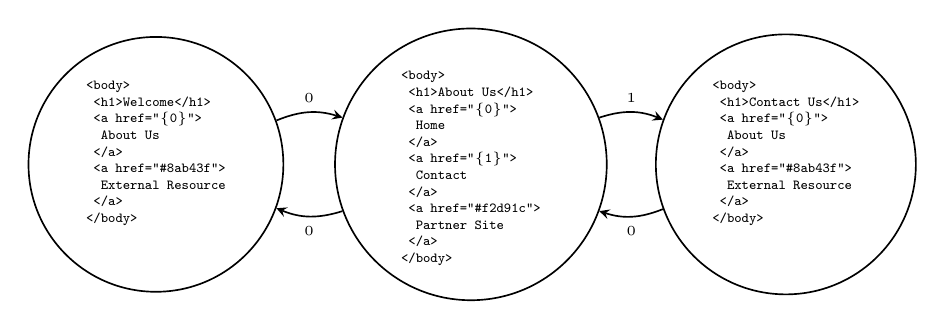
\begin{tikzpicture}[
    > = stealth, % arrow head style
    node distance=4cm,
    every node/.style={draw, align=left, font=\tiny},
    semithick % line style
]

% Nodes
\node[state] (index) {\\ \texttt{<body>} \\ \texttt{ <h1>Welcome</h1>} \\ \texttt{ <a href="\{0\}">} \\ \texttt{ ~About Us} \\ \texttt{ </a>} \\ \texttt{ <a href="\#8ab43f">} \\ \texttt{ ~External Resource} \\ \texttt{ </a>} \\ \texttt{</body>} \\ \\};
\node[state] (about) [right of=index] { \\ \texttt{<body>} \\ \texttt{ <h1>About Us</h1>} \\ \texttt{ <a href="\{0\}">} \\ \texttt{ ~Home} \\ \texttt{ </a>} \\ \texttt{ <a href="\{1\}">} \\ \texttt{ ~Contact} \\ \texttt{ </a>} \\ \texttt{ <a href="\#f2d91c">} \\ \texttt{ ~Partner Site} \\ \texttt{ </a>} \\ \texttt{</body>}};
\node[state] (contact) [right of= about] {\\ \texttt{<body>} \\ \texttt{ <h1>Contact Us</h1>} \\ \texttt{ <a href="\{0\}">} \\ \texttt{ ~About Us} \\ \texttt{ </a>} \\ \texttt{ <a href="\#8ab43f">} \\ \texttt{ ~External Resource} \\ \texttt{ </a>} \\ \texttt{</body>} \\ \\};

% Edges (internal links only)
\draw[->] (index) to[bend left=20] node[above, draw=none] {0} (about);
\draw[->] (about) to[bend left=20] node[below, draw=none] {0} (index);
\draw[->] (about) to[bend left=20] node[above, draw=none] {1} (contact);
\draw[->] (contact) to[bend left=20] node[below, draw=none] {0} (about);

\end{tikzpicture}

\caption{Visualization of procedure for hashing a three page HTML website. Note that in Row 2, the values \#8ab43f and \#f2d91c refer to hashes computed recursively - in this case the hash of pages on external websites.}

%Visualization of web page link structure: (Row 1) Original HTML with URLs, (Row 2) Tokenized version with internal links as \{n\} and external links as hash codes, (Row 3) Directed graph showing internal link structure with node labels corresponding to tokenized identifiers.}
\end{figure}

From the algorithms given so far, it may not be obvious how to implement these graph theoretic procedures for real world data. Here we will discuss how to do so by taking the example of a static hyperlinked web page system stored in a content addressed distributed hash table (DHT).

In this sketch, we will assume that our web pages are static HTML files which link to each other and to external websites. These files form a directed graph where each page is a node, and links between pages are edges. The outgoing edges from a node are labeled by natural numbers in the order in which the links appear in the HTML file. Figure \ref{fig:webpage-example} gives a concrete example of the process described here.

We begin by considering the links within each file and the strongly connected components created by our website. All intra-SCC links are replaced with natural numbers in the order in which the links appear. Links leaving the SCC are recursively hashed, and these hash values are inserted verbatim into the HTML of our webpages. We then compute the canonical order and orbit partition of the SCC in polynomial time using Algorithm \ref{alg:scc-outgoing-edges}.

We then insert the SCC into the DHT as follows:
\begin{itemize}
  \item \textbf{Key}: The hash of the SCC computed via Algorithm \ref{digraphhash}.
  \item \textbf{Value}: The canonized adjacency list and the label list (which is ordered in the canonical order).
\end{itemize}

For each page in the SCC, we insert the following into the DHT:

\begin{itemize}
  \item \textbf{Key}: The string hash of the (orbit index, SCC hash). We compute the orbit index as is done so in Algorithm \ref{digraphnodehash}.
  \item \textbf{Value}: The (orbit index, SCC hash) pair.
\end{itemize}

Suppose that a user wants to navigate our website, and has obtained a hash for one specific page. The browser software will begin by retrieving the orbit index and SCC hash from our distributed hash table (DHT). The browser then retrieves the SCC, giving us the adjacency list and allowing the SCC digraph to be reconstructed. The orbit index will then point us to a specific node in the SCC. The browser will display the contents of this node to the user.

If the user clicks a link within the same SCC, the browser simply follows the graph edge and shows the appropriate page contents. For links that leave the SCC, the browser repeats the same process from the beginning, retrieving the new SCC from the DHT.

\section{Related Work}

\section{Experimental Results}

%
% ---- Bibliography ----
%
%\begin{thebibliography}{6}
%

%\bibitem {bib1}
%Smith, T.F., Waterman, M.S.: Identification of common molecular subsequences.
%J. Mol. Biol. 147, 195?197 (1981). \url{doi:10.1016/0022-2836(81)90087-5}

%\bibitem {may:ehr:stein}
%May, P., Ehrlich, H.-C., Steinke, T.: ZIB structure prediction pipeline:
%composing a complex biological workflow through web services.
%In: Nagel, W.E., Walter, W.V., Lehner, W. (eds.) Euro-Par 2006.
%LNCS, vol. 4128, pp. 1148?1158. Springer, Heidelberg (2006).
%\url{doi:10.1007/11823285_121}

%\bibitem {fost:kes}
%Foster, I., Kesselman, C.: The Grid: Blueprint for a New Computing Infrastructure.
%Morgan Kaufmann, San Francisco (1999)

%\bibitem {czaj:fitz}
%Czajkowski, K., Fitzgerald, S., Foster, I., Kesselman, C.: Grid information services
%for distributed resource sharing. In: 10th IEEE International Symposium
%on High Performance Distributed Computing, pp. 181?184. IEEE Press, New York (2001).
%\url{doi: 10.1109/HPDC.2001.945188}

%\bibitem {fo:kes:nic:tue}
%Foster, I., Kesselman, C., Nick, J., Tuecke, S.: The physiology of the grid: an open grid services architecture for distributed systems integration. Technical report, Global Grid
%Forum (2002)

%\bibitem {onlyurl}
%National Center for Biotechnology Information. \url{http://www.ncbi.nlm.nih.gov}

%\end{thebibliography}

% ---- OR ------- Uncomment this section to use bibtex
\bibliographystyle{spmpsci} % We choose the "plain" reference style
\bibliography{refs} % Entries are in the refs.bib file
\end{document}
